% Options for packages loaded elsewhere
\PassOptionsToPackage{unicode}{hyperref}
\PassOptionsToPackage{hyphens}{url}
\documentclass[
  12 pt,
]{article}
\usepackage{xcolor}
\usepackage[margin = 1.0in]{geometry}
\usepackage{amsmath,amssymb}
\setcounter{secnumdepth}{-\maxdimen} % remove section numbering
\usepackage{iftex}
\ifPDFTeX
  \usepackage[T1]{fontenc}
  \usepackage[utf8]{inputenc}
  \usepackage{textcomp} % provide euro and other symbols
\else % if luatex or xetex
  \usepackage{unicode-math} % this also loads fontspec
  \defaultfontfeatures{Scale=MatchLowercase}
  \defaultfontfeatures[\rmfamily]{Ligatures=TeX,Scale=1}
\fi
\usepackage{lmodern}
\ifPDFTeX\else
  % xetex/luatex font selection
\fi
% Use upquote if available, for straight quotes in verbatim environments
\IfFileExists{upquote.sty}{\usepackage{upquote}}{}
\IfFileExists{microtype.sty}{% use microtype if available
  \usepackage[]{microtype}
  \UseMicrotypeSet[protrusion]{basicmath} % disable protrusion for tt fonts
}{}
\makeatletter
\@ifundefined{KOMAClassName}{% if non-KOMA class
  \IfFileExists{parskip.sty}{%
    \usepackage{parskip}
  }{% else
    \setlength{\parindent}{0pt}
    \setlength{\parskip}{6pt plus 2pt minus 1pt}}
}{% if KOMA class
  \KOMAoptions{parskip=half}}
\makeatother
\usepackage{longtable,booktabs,array}
\usepackage{calc} % for calculating minipage widths
% Correct order of tables after \paragraph or \subparagraph
\usepackage{etoolbox}
\makeatletter
\patchcmd\longtable{\par}{\if@noskipsec\mbox{}\fi\par}{}{}
\makeatother
% Allow footnotes in longtable head/foot
\IfFileExists{footnotehyper.sty}{\usepackage{footnotehyper}}{\usepackage{footnote}}
\makesavenoteenv{longtable}
\usepackage{graphicx}
\makeatletter
\newsavebox\pandoc@box
\newcommand*\pandocbounded[1]{% scales image to fit in text height/width
  \sbox\pandoc@box{#1}%
  \Gscale@div\@tempa{\textheight}{\dimexpr\ht\pandoc@box+\dp\pandoc@box\relax}%
  \Gscale@div\@tempb{\linewidth}{\wd\pandoc@box}%
  \ifdim\@tempb\p@<\@tempa\p@\let\@tempa\@tempb\fi% select the smaller of both
  \ifdim\@tempa\p@<\p@\scalebox{\@tempa}{\usebox\pandoc@box}%
  \else\usebox{\pandoc@box}%
  \fi%
}
% Set default figure placement to htbp
\def\fps@figure{htbp}
\makeatother
\setlength{\emergencystretch}{3em} % prevent overfull lines
\providecommand{\tightlist}{%
  \setlength{\itemsep}{0pt}\setlength{\parskip}{0pt}}
%%%%%%%%%%%%%%%%%%%%%%%%%%%%%%%%%%%%%%%%%%%%%%%%%%%%%%%%%%%%
% Font
%%%%%%%%%%%%%%%%%%%%%%%%%%%%%%%%%%%%%%%%%%%%%%%%%%%%%%%%%%%%

% Set font encoding to T1 (8-bit encoding, 256 glyphs) 
% (improved text handling, especially with non-English
% languages and text containing special characters)
\usepackage[T1]{fontenc}

% Set font to URW Nimbus Roman
% (Times New Roman alternative)
\usepackage{mathptmx}

%%%%%%%%%%%%%%%%%%%%%%%%%%%%%%%%%%%%%%%%%%%%%%%%%%%%%%%%%%%%
% Typsetting
%%%%%%%%%%%%%%%%%%%%%%%%%%%%%%%%%%%%%%%%%%%%%%%%%%%%%%%%%%%%

% Include the package containing commands for page
% orientation
\usepackage{pdflscape}
% Create a new custom command for starting a landscape block
\newcommand{\blandscape}{\begin{landscape}}
% Create a new custom command for ending a landscape block
\newcommand{\elandscape}{\end{landscape}}

% Include package providing fine-tuned typographic
% enhancements
\usepackage{microtype}

% Suppress hyphenation
\usepackage[none]{hyphenat}

% Include package for setting spacing between lines
\usepackage{setspace}
% Set line spacing
\doublespacing

% Indent first paragraph of each section (including
% chapters)
\usepackage{indentfirst}

% Set vertical space between paragraphs
\setlength{\parskip}{1em}

%%%%%%%%%%%%%%%%%%%%%%%%%%%%%%%%%%%%%%%%%%%%%%%%%%%%%%%%%%%%
% Line numbers
%%%%%%%%%%%%%%%%%%%%%%%%%%%%%%%%%%%%%%%%%%%%%%%%%%%%%%%%%%%%

% Include package for line numbering
\usepackage{lineno}
% Set font style and size of line numbers
\renewcommand{\linenumberfont}{\normalfont\tiny}

%%%%%%%%%%%%%%%%%%%%%%%%%%%%%%%%%%%%%%%%%%%%%%%%%%%%%%%%%%%%
% Lists
%%%%%%%%%%%%%%%%%%%%%%%%%%%%%%%%%%%%%%%%%%%%%%%%%%%%%%%%%%%%

% Include package to customise the appearance of itemised
% lists
\usepackage{enumitem}

% Remove extra vertical space that is added above and below
% itemize and enumerate lists
\setlist{nosep}

%%%%%%%%%%%%%%%%%%%%%%%%%%%%%%%%%%%%%%%%%%%%%%%%%%%%%%%%%%%%
% Figures and tables
%%%%%%%%%%%%%%%%%%%%%%%%%%%%%%%%%%%%%%%%%%%%%%%%%%%%%%%%%%%%

% Include package enhancing figure and table placement
% (provides "H" placement specifier forcing the float to
% appear exactly where it is defined)
\usepackage{float}

% Include package used to create tables with cells spanning
% multiple rows
\usepackage{multirow}

%%%%%%%%%%%%%%%%%%%%%%%%%%%%%%%%%%%%%%%%%%%%%%%%%%%%%%%%%%%%
% Captions
%%%%%%%%%%%%%%%%%%%%%%%%%%%%%%%%%%%%%%%%%%%%%%%%%%%%%%%%%%%%

% Define the separator between the label and the caption
% text and make the label bold
\usepackage[labelsep=space, labelfont=bf]{caption}
% Set caption text to be justified
\captionsetup{justification=justified}

%%%%%%%%%%%%%%%%%%%%%%%%%%%%%%%%%%%%%%%%%%%%%%%%%%%%%%%%%%%%
% Uniform Resource Locators (URLs)
%%%%%%%%%%%%%%%%%%%%%%%%%%%%%%%%%%%%%%%%%%%%%%%%%%%%%%%%%%%%

% Include the package to handle URLs
\usepackage{url}

% Redefine the commands that specify where line breaks can
% occur in URLs (\UrlBreaks has a lower penalty, i.e. it is
% more easily chosen, and does not break within a repeating
% sequence)
\renewcommand\UrlBreaks{\do\/\do\:\do\.\do\-}
\renewcommand\UrlBigBreaks{\do\/\do\:\do\.\do\-}

%%%%%%%%%%%%%%%%%%%%%%%%%%%%%%%%%%%%%%%%%%%%%%%%%%%%%%%%%%%%
% Referencing
%%%%%%%%%%%%%%%%%%%%%%%%%%%%%%%%%%%%%%%%%%%%%%%%%%%%%%%%%%%%

% Include the package xr (external references) to allow
% referencing labels from another file
\usepackage{xr}
% Specify the name of the file used for additional
% referencing and define the prefix for the labels
% from the external document
\externaldocument[supp-]{supplementary}

%%%%%%%%%%%%%%%%%%%%%%%%%%%%%%%%%%%%%%%%%%%%%%%%%%%%%%%%%%%%
% Measurement units
%%%%%%%%%%%%%%%%%%%%%%%%%%%%%%%%%%%%%%%%%%%%%%%%%%%%%%%%%%%%

% Include the package that facilitates consistent formatting
% of scientific units and numbers
\usepackage{siunitx}
% Define unit \molar as moles per cubic decimetre
\DeclareSIUnit\molar{\mole\per\cubic\deci\metre}
% Define unit \Molar as small caps "M"
\DeclareSIUnit\Molar{\textsc{m}}
% Define unit \cells as the text "cells"
\DeclareSIUnit\cells{\text{cells}}
% Define unit \litre as lower case "l"
\DeclareSIUnit\litre{l}
% Define unit \vV as v/v
\DeclareSIUnit{\vV}{v/v}
% Define unit \wW as w/w
\DeclareSIUnit{\wW}{w/w}
% Define unit \bp as bp
\DeclareSIUnit{\bp}{bp}
% Define unit \U as U
\DeclareSIUnit{\U}{U}
% Remove the space between the number and the percentage
% sign
\catcode`\%=12\relax
\DeclareSIUnit[number-unit-product = ]\percent{%}
\catcode`\%=14\relax

%%%%%%%%%%%%%%%%%%%%%%%%%%%%%%%%%%%%%%%%%%%%%%%%%%%%%%%%%%%%
% Chemical formulas
%%%%%%%%%%%%%%%%%%%%%%%%%%%%%%%%%%%%%%%%%%%%%%%%%%%%%%%%%%%%

% Include package for typesetting chemical formulas
\usepackage{chemformula}

%%%%%%%%%%%%%%%%%%%%%%%%%%%%%%%%%%%%%%%%%%%%%%%%%%%%%%%%%%%%
% Bookmarks
%%%%%%%%%%%%%%%%%%%%%%%%%%%%%%%%%%%%%%%%%%%%%%%%%%%%%%%%%%%%

% Include package to create hyperlinks, including PDF bookmarks, and
% open all levels of the bookmarks by default
\usepackage[bookmarksopenlevel=\maxdimen]{hyperref}

\usepackage{bookmark}
\IfFileExists{xurl.sty}{\usepackage{xurl}}{} % add URL line breaks if available
\urlstyle{same}
\hypersetup{
  pdftitle={Supplementary material},
  hidelinks,
  pdfcreator={LaTeX via pandoc}}

\title{\textbf{Supplementary material}}
\usepackage{etoolbox}
\makeatletter
\providecommand{\subtitle}[1]{% add subtitle to \maketitle
  \apptocmd{\@title}{\par {\large #1 \par}}{}{}
}
\makeatother
\subtitle{\textbf{Resident and transient microbial taxa in the gill microbiome of the mussel \emph{Mytilus galloprovincialis}}}
\author{}
\date{\vspace{-2.5em}}

\begin{document}
\maketitle

%%%%%%%%%%%%%%%%%%%%%%%%%%%%%%%%%%%%%%%%%%%%%%%%%%%%%%%%%%%%
% Captions
%%%%%%%%%%%%%%%%%%%%%%%%%%%%%%%%%%%%%%%%%%%%%%%%%%%%%%%%%%%%

% Set the name for figures to "Supplementary Figure"
\renewcommand{\figurename}{Supplementary Fig.}
% Set the name for tables to "Supplementary Table"
\renewcommand{\tablename}{Supplementary Table}
% Use Arabic numerals to number figures and format
% figure caption numbers as S1, S2, S3, and so on
\renewcommand{\thefigure}{S\arabic{figure}}
% Use Arabic numerals to number tables and format
% table caption numbers as S1, S2, S3, and so on
\renewcommand{\thetable}{S\arabic{table}}


\vspace{\fill}

Marino Korlević\textsuperscript{1*}, Marsej Markovski\textsuperscript{1}, Damir Kapetanović\textsuperscript{2}, Irena Vardić Smrzlić\textsuperscript{2}, Karla Orlić\textsuperscript{2}, Jakša Bolotin\textsuperscript{3}, Valter Kožul\textsuperscript{3}, Svjetlana Bobanović-Ćolić\textsuperscript{3}, Vedrana Nerlović\textsuperscript{4}, and Lorena Perić\textsuperscript{2*}

\begin{enumerate}
\def\labelenumi{\arabic{enumi}.}
\tightlist
\item
  Centre for Marine Research, Ruđer Bošković Institute, Croatia
\item
  Division for Marine and Environmental Research, Ruđer Bošković Institute, Croatia
\item
  Institute for Marine and Coastal Research, University of Dubrovnik, Croatia
\item
  Faculty of Marine Sciences, University of Split, Croatia
\end{enumerate}

\textsuperscript{*}To whom correspondence should be addressed:\\
Marino Korlević\\
G. Paliaga 5, 52210 Rovinj, Croatia\\
e-mail: \href{mailto:marino.korlevic@irb.hr}{\nolinkurl{marino.korlevic@irb.hr}}\\
ORCID iD: \href{https://orcid.org/0000-0001-5680-3556}{0000-0001-5680-3556}

Lorena Perić\\
Bijenička cesta 54, 10000 Zagreb, Croatia\\
e-mail: \href{mailto:lorena.peric@irb.hr}{\nolinkurl{lorena.peric@irb.hr}}\\
ORCID iD: \href{https://orcid.org/0000-0001-6899-9605}{0000-0001-6899-9605}

% Ensure that numbers are typeset in text mode
\sisetup{mode=text}

% Set the size of indentation to 24 pt
\setlength\parindent{24pt}

% Start a new page
\newpage

% Begin landscape orientation
\blandscape

\subsection{Supplementary figures}\label{supplementary-figures}

\begin{figure}[H]

{\centering 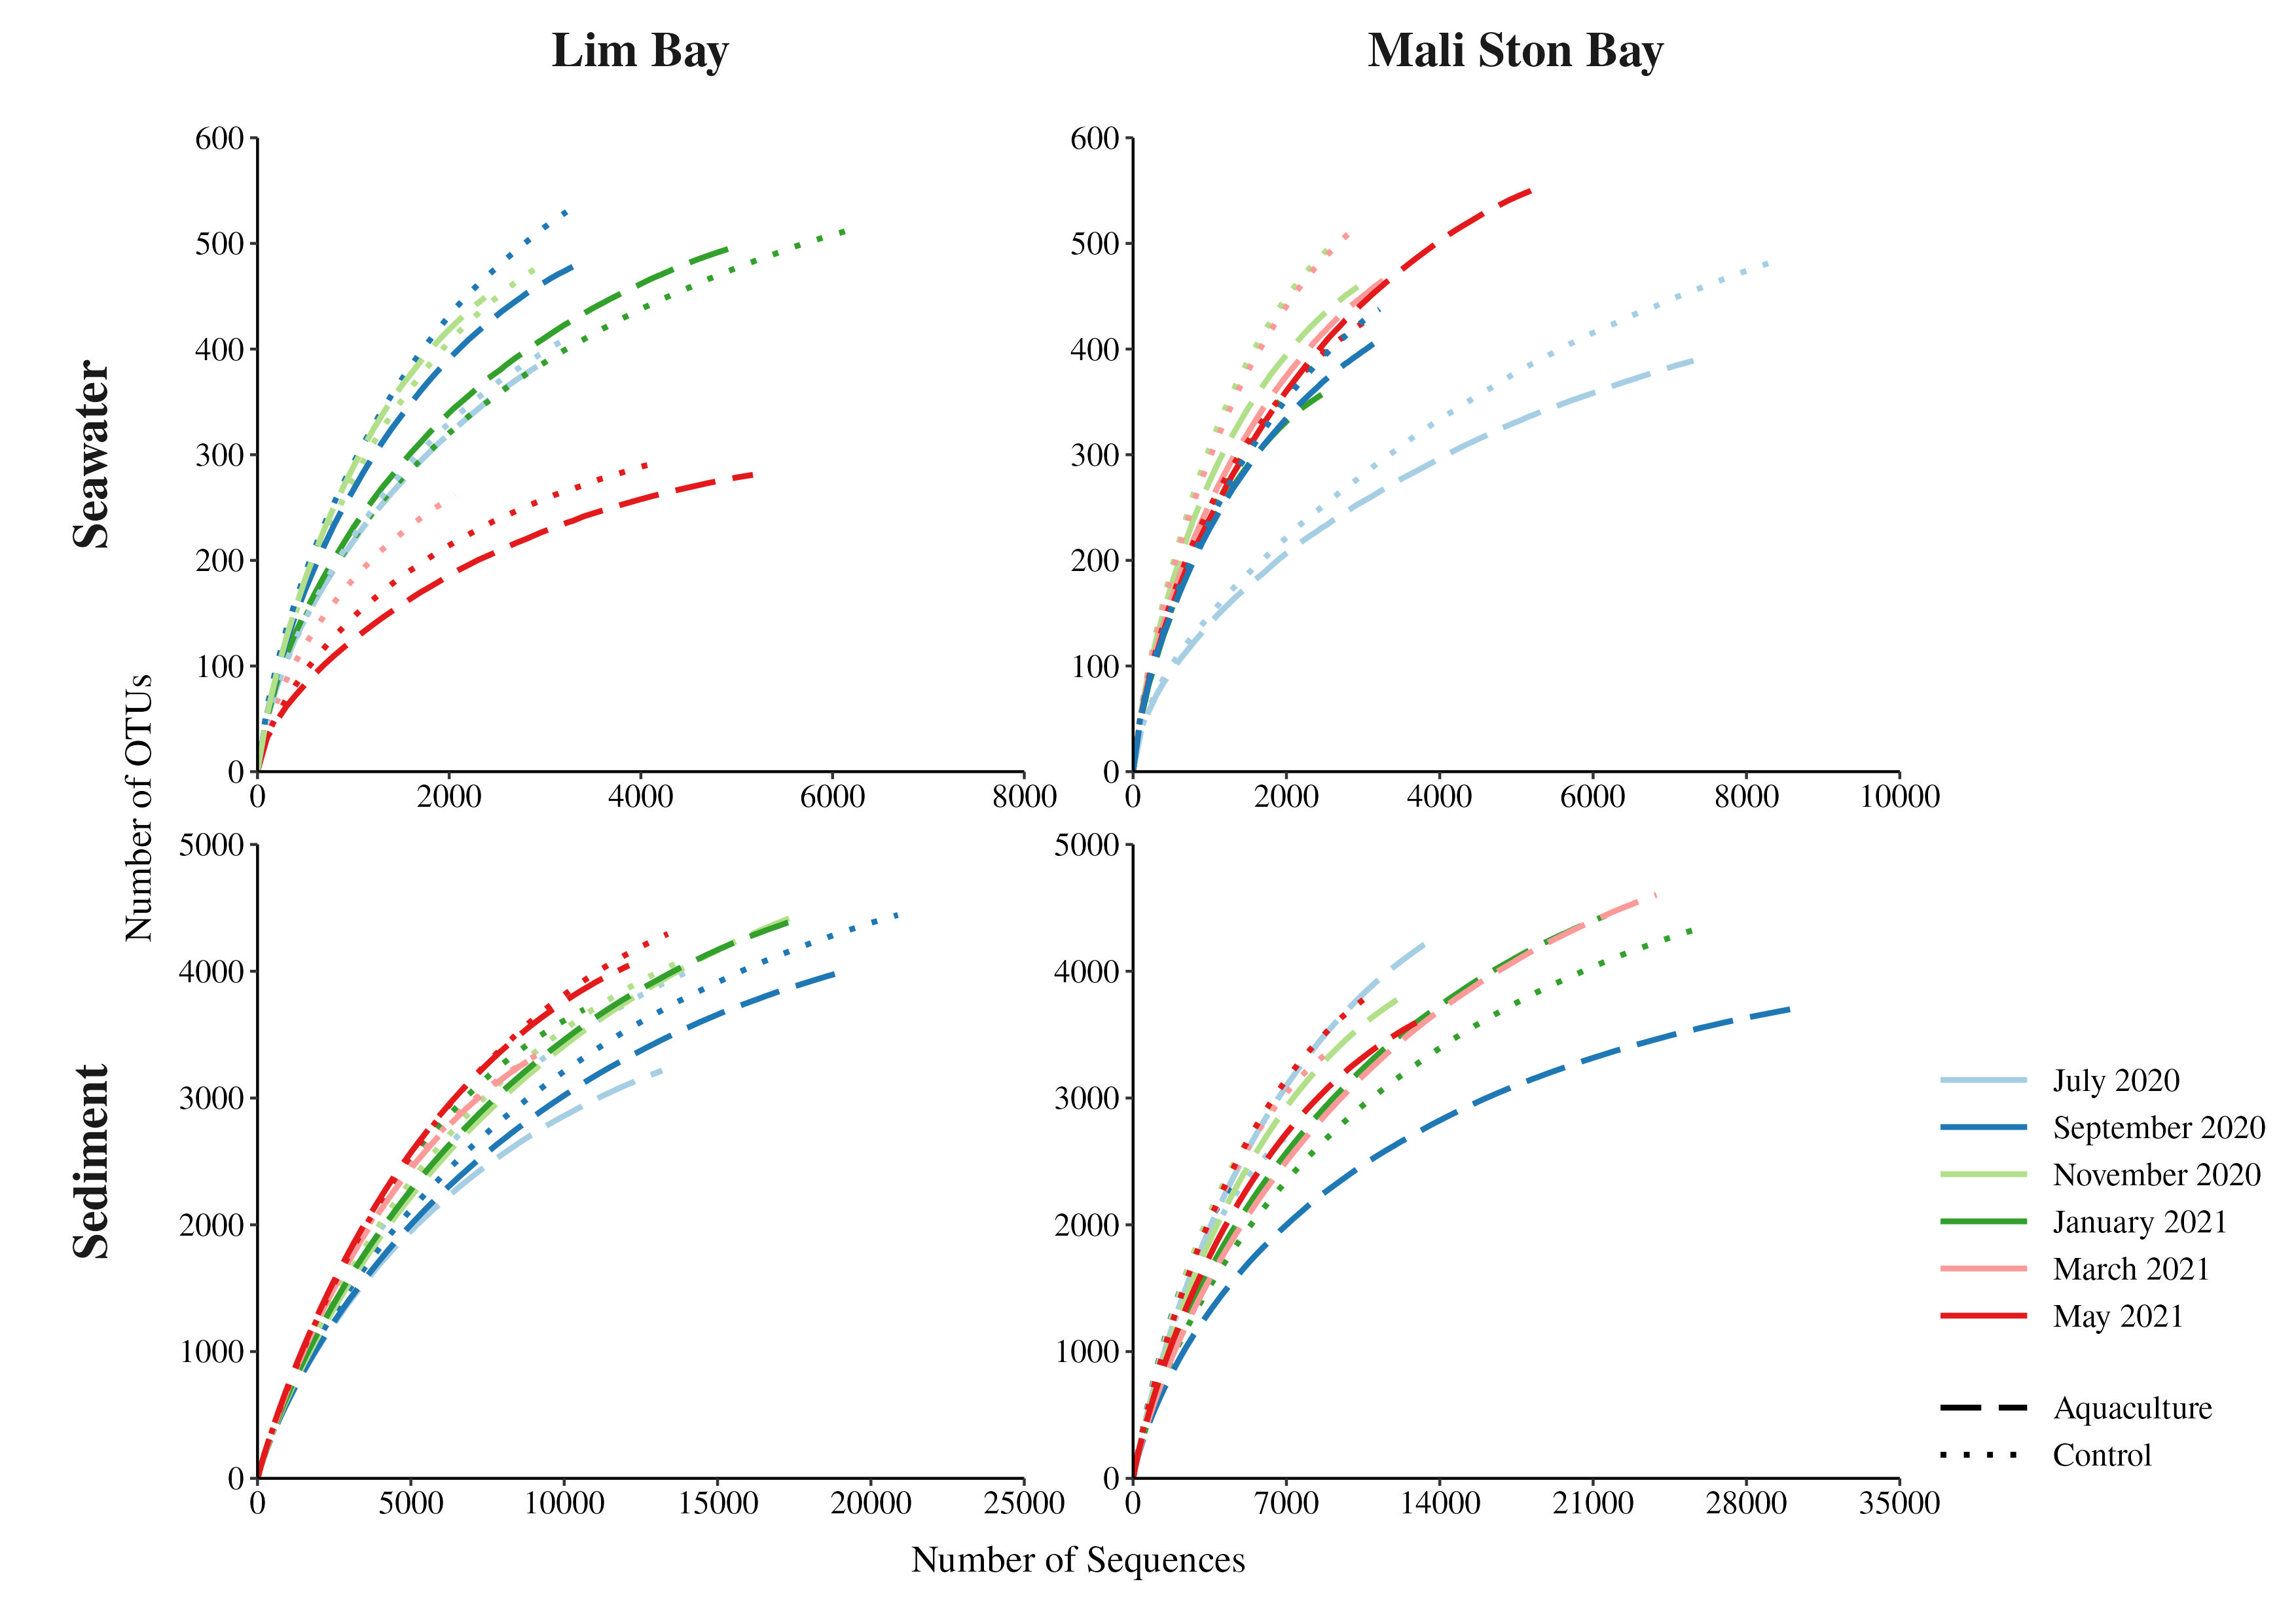
\includegraphics[width=0.85\linewidth]{../results/figures/rarefaction_a} 

}

\caption{Rarefaction curves of seawater and sediment microbial communities sampled in Lim Bay and Mali Ston Bay from July 2020 to May 2021. In each bay, samples were collected from one aquaculture site and one control site}\label{fig:rarefaction-a}
\end{figure}



% End landscape orientation
\elandscape

\begin{figure}[H]

{\centering 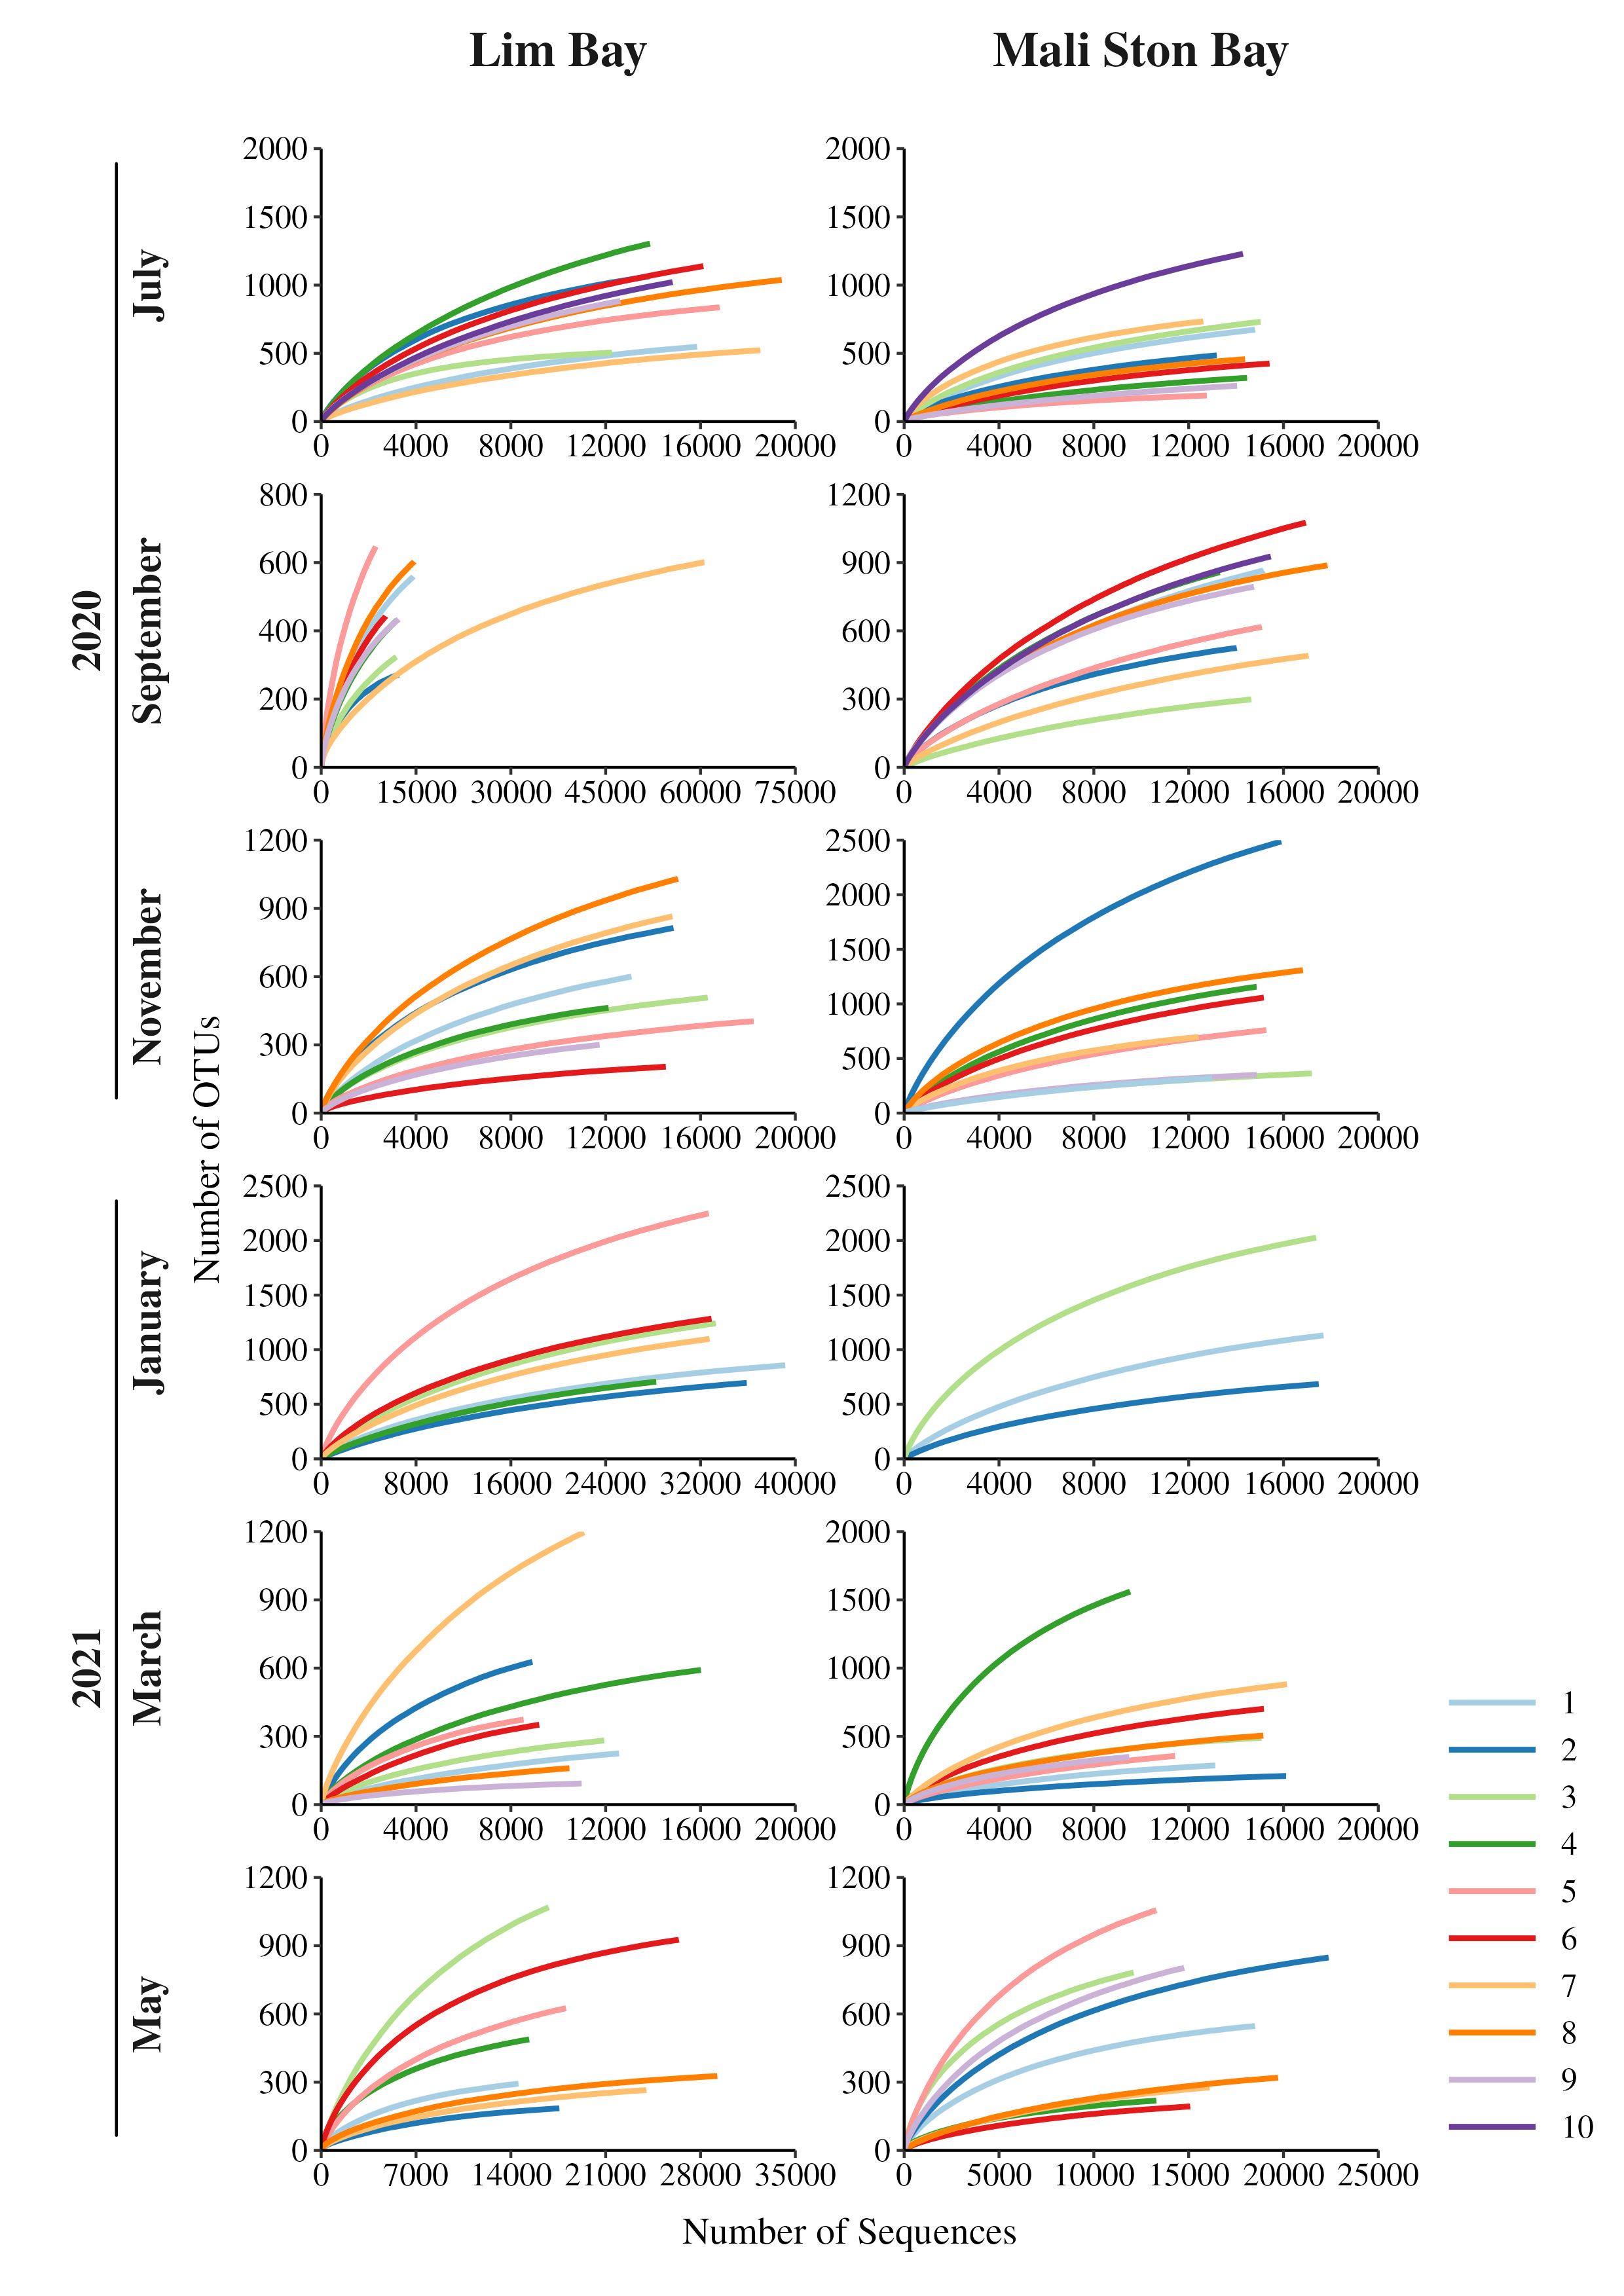
\includegraphics[width=0.85\linewidth]{../results/figures/rarefaction_b} 

}

\caption{Rarefaction curves of microbial communities associated with the gills of the mussel \emph{M. galloprovincialis} (gill microbiome). Mussels were collected in Lim Bay and Mali Ston Bay from July 2020 to May 2021. The numbers in the legend correspond to the index of each individual mussel}\label{fig:rarefaction-b}
\end{figure}



\begin{figure}[H]

{\centering 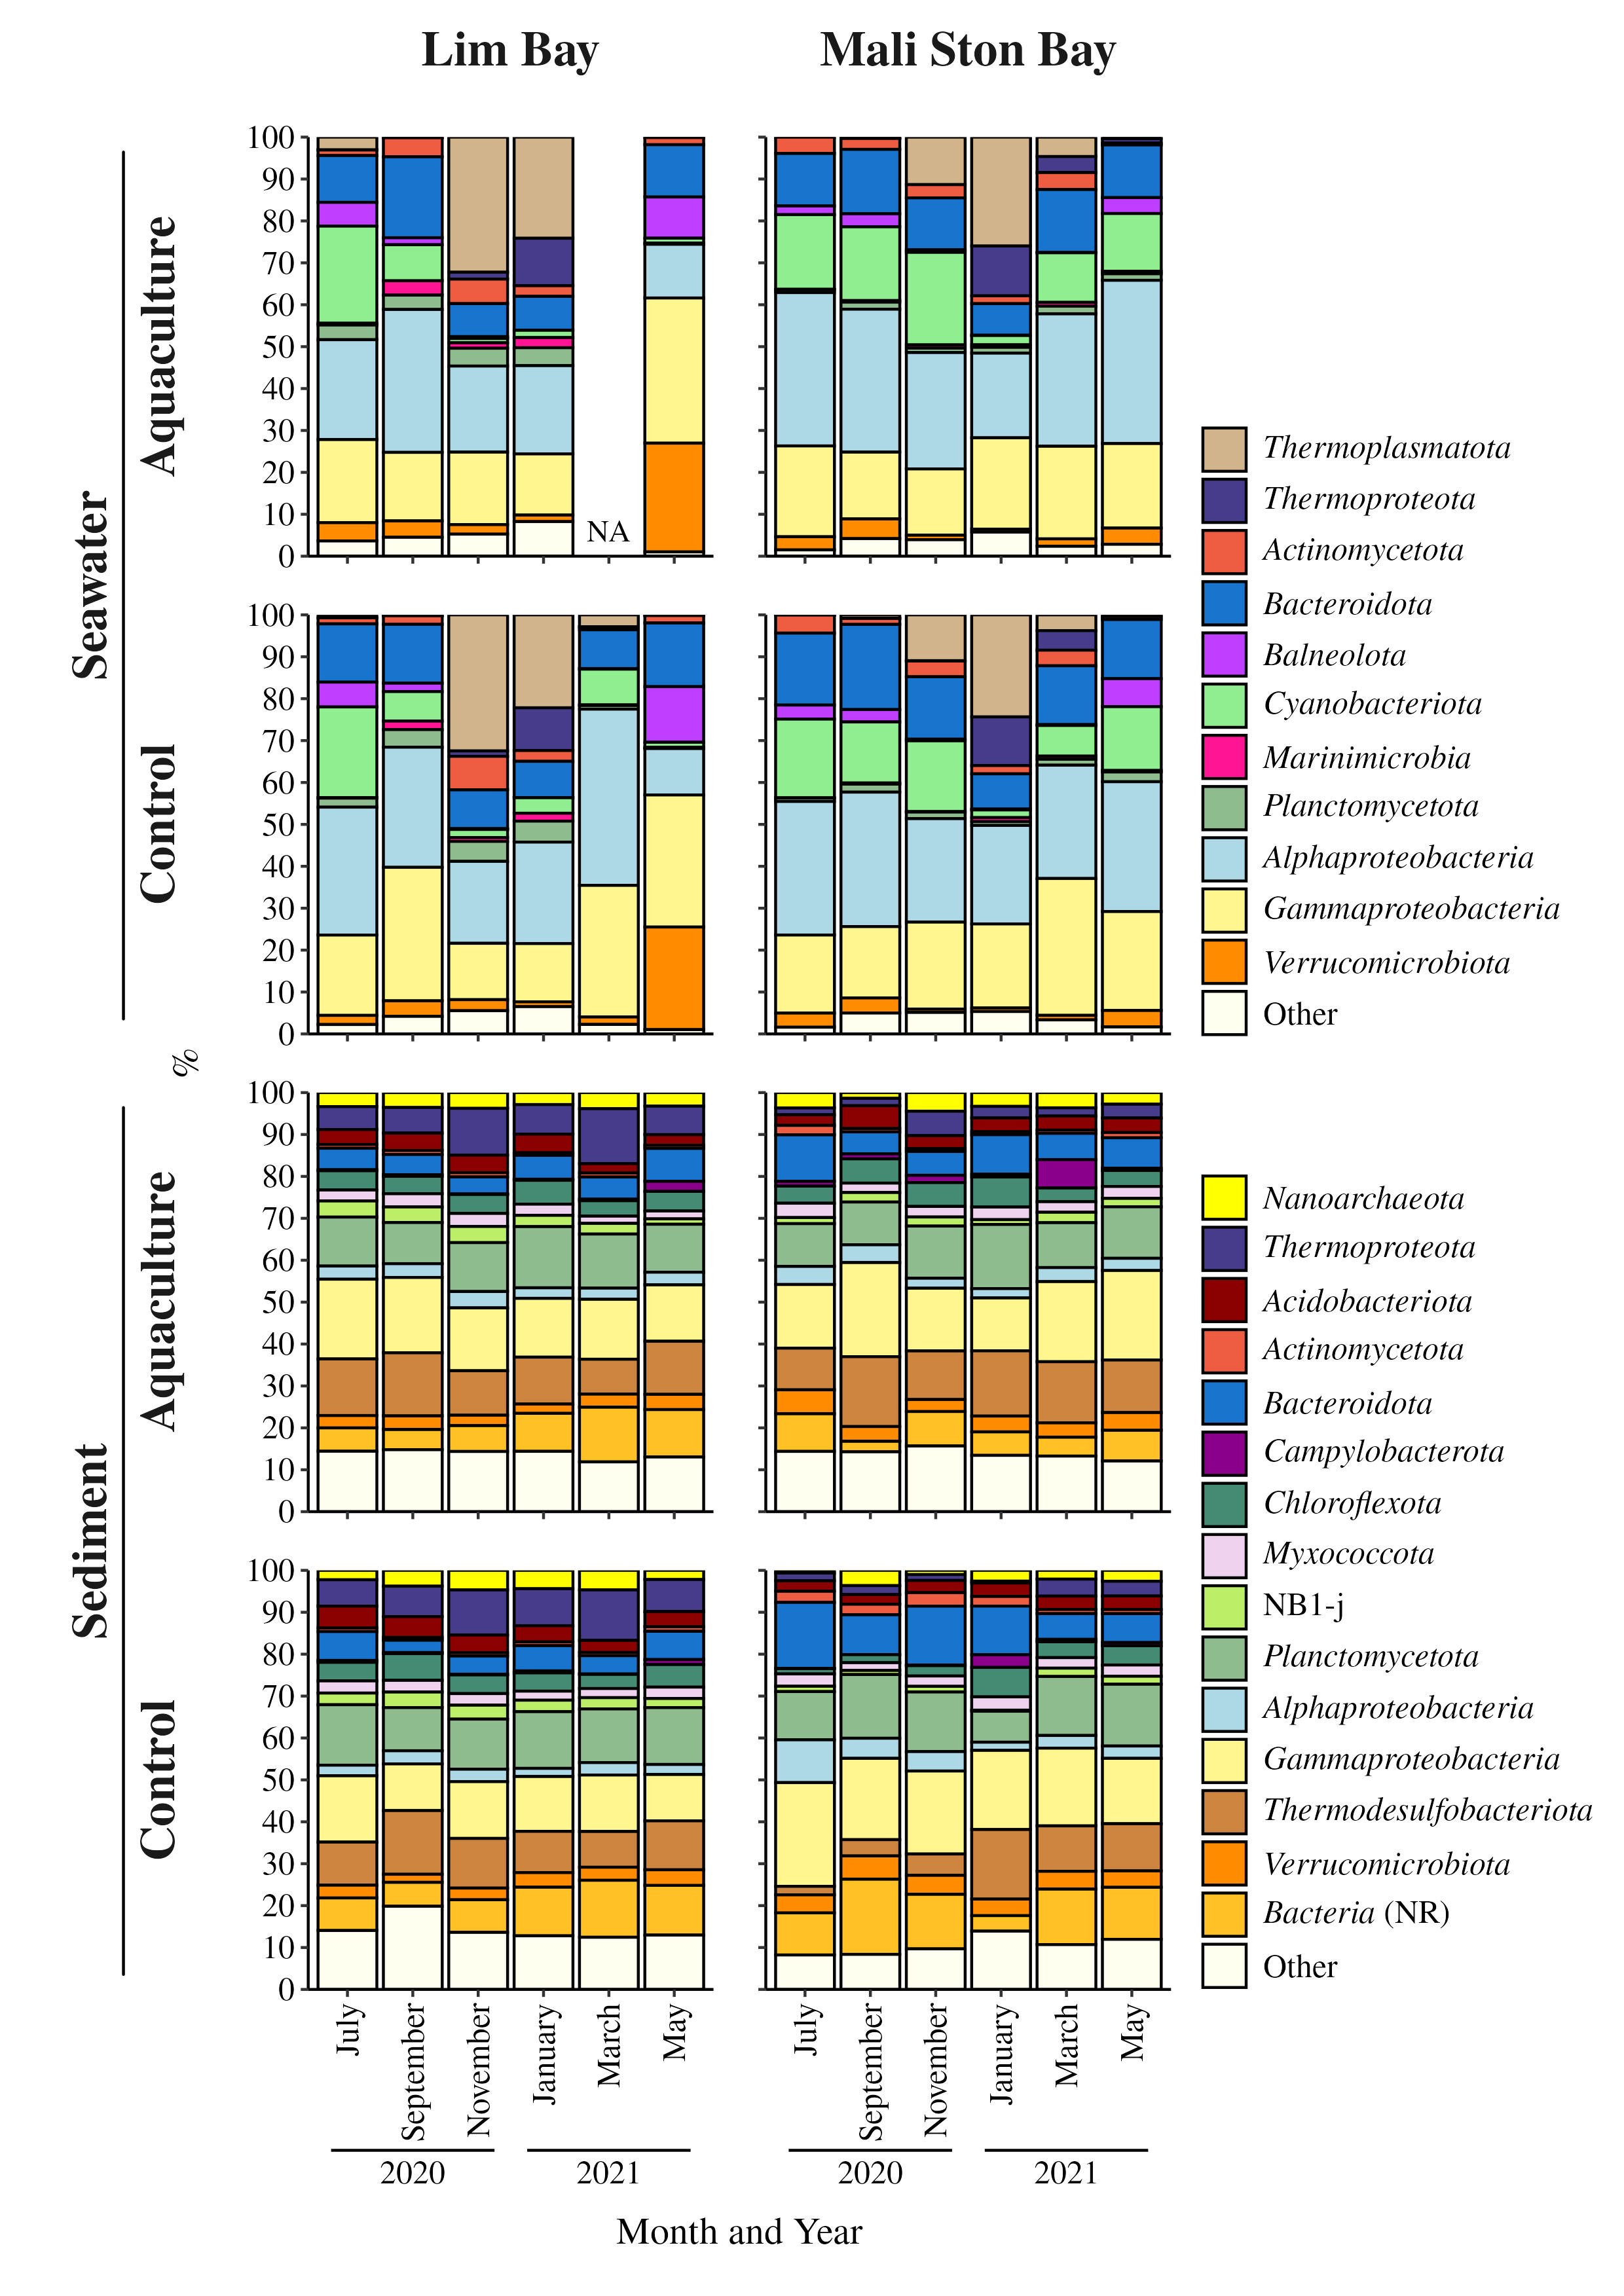
\includegraphics[width=0.8\linewidth]{../results/figures/taxonomy_seawater_sediment_phylum} 

}

\caption{Taxonomic classification and relative contribution of the most abundant (\qty{>=3}{\percent}) bacterial and archaeal sequences in the seawater and sediment of Lim Bay and Mali Ston Bay. In each bay, samples were collected from one aquaculture site and one control site between July 2020 and May 2021. ``No Relative'' indicates sequences that could not be classified into any taxon, while ``NR'' (No Relative) next to the name of a taxonomic group refers to sequences that could not be assigned to any known taxon within that group. ``NA'' (Not Available) indicates samples that were not successfully analysed}\label{fig:taxonomy-seawater-sediment-phylum}
\end{figure}



\begin{figure}[H]

{\centering 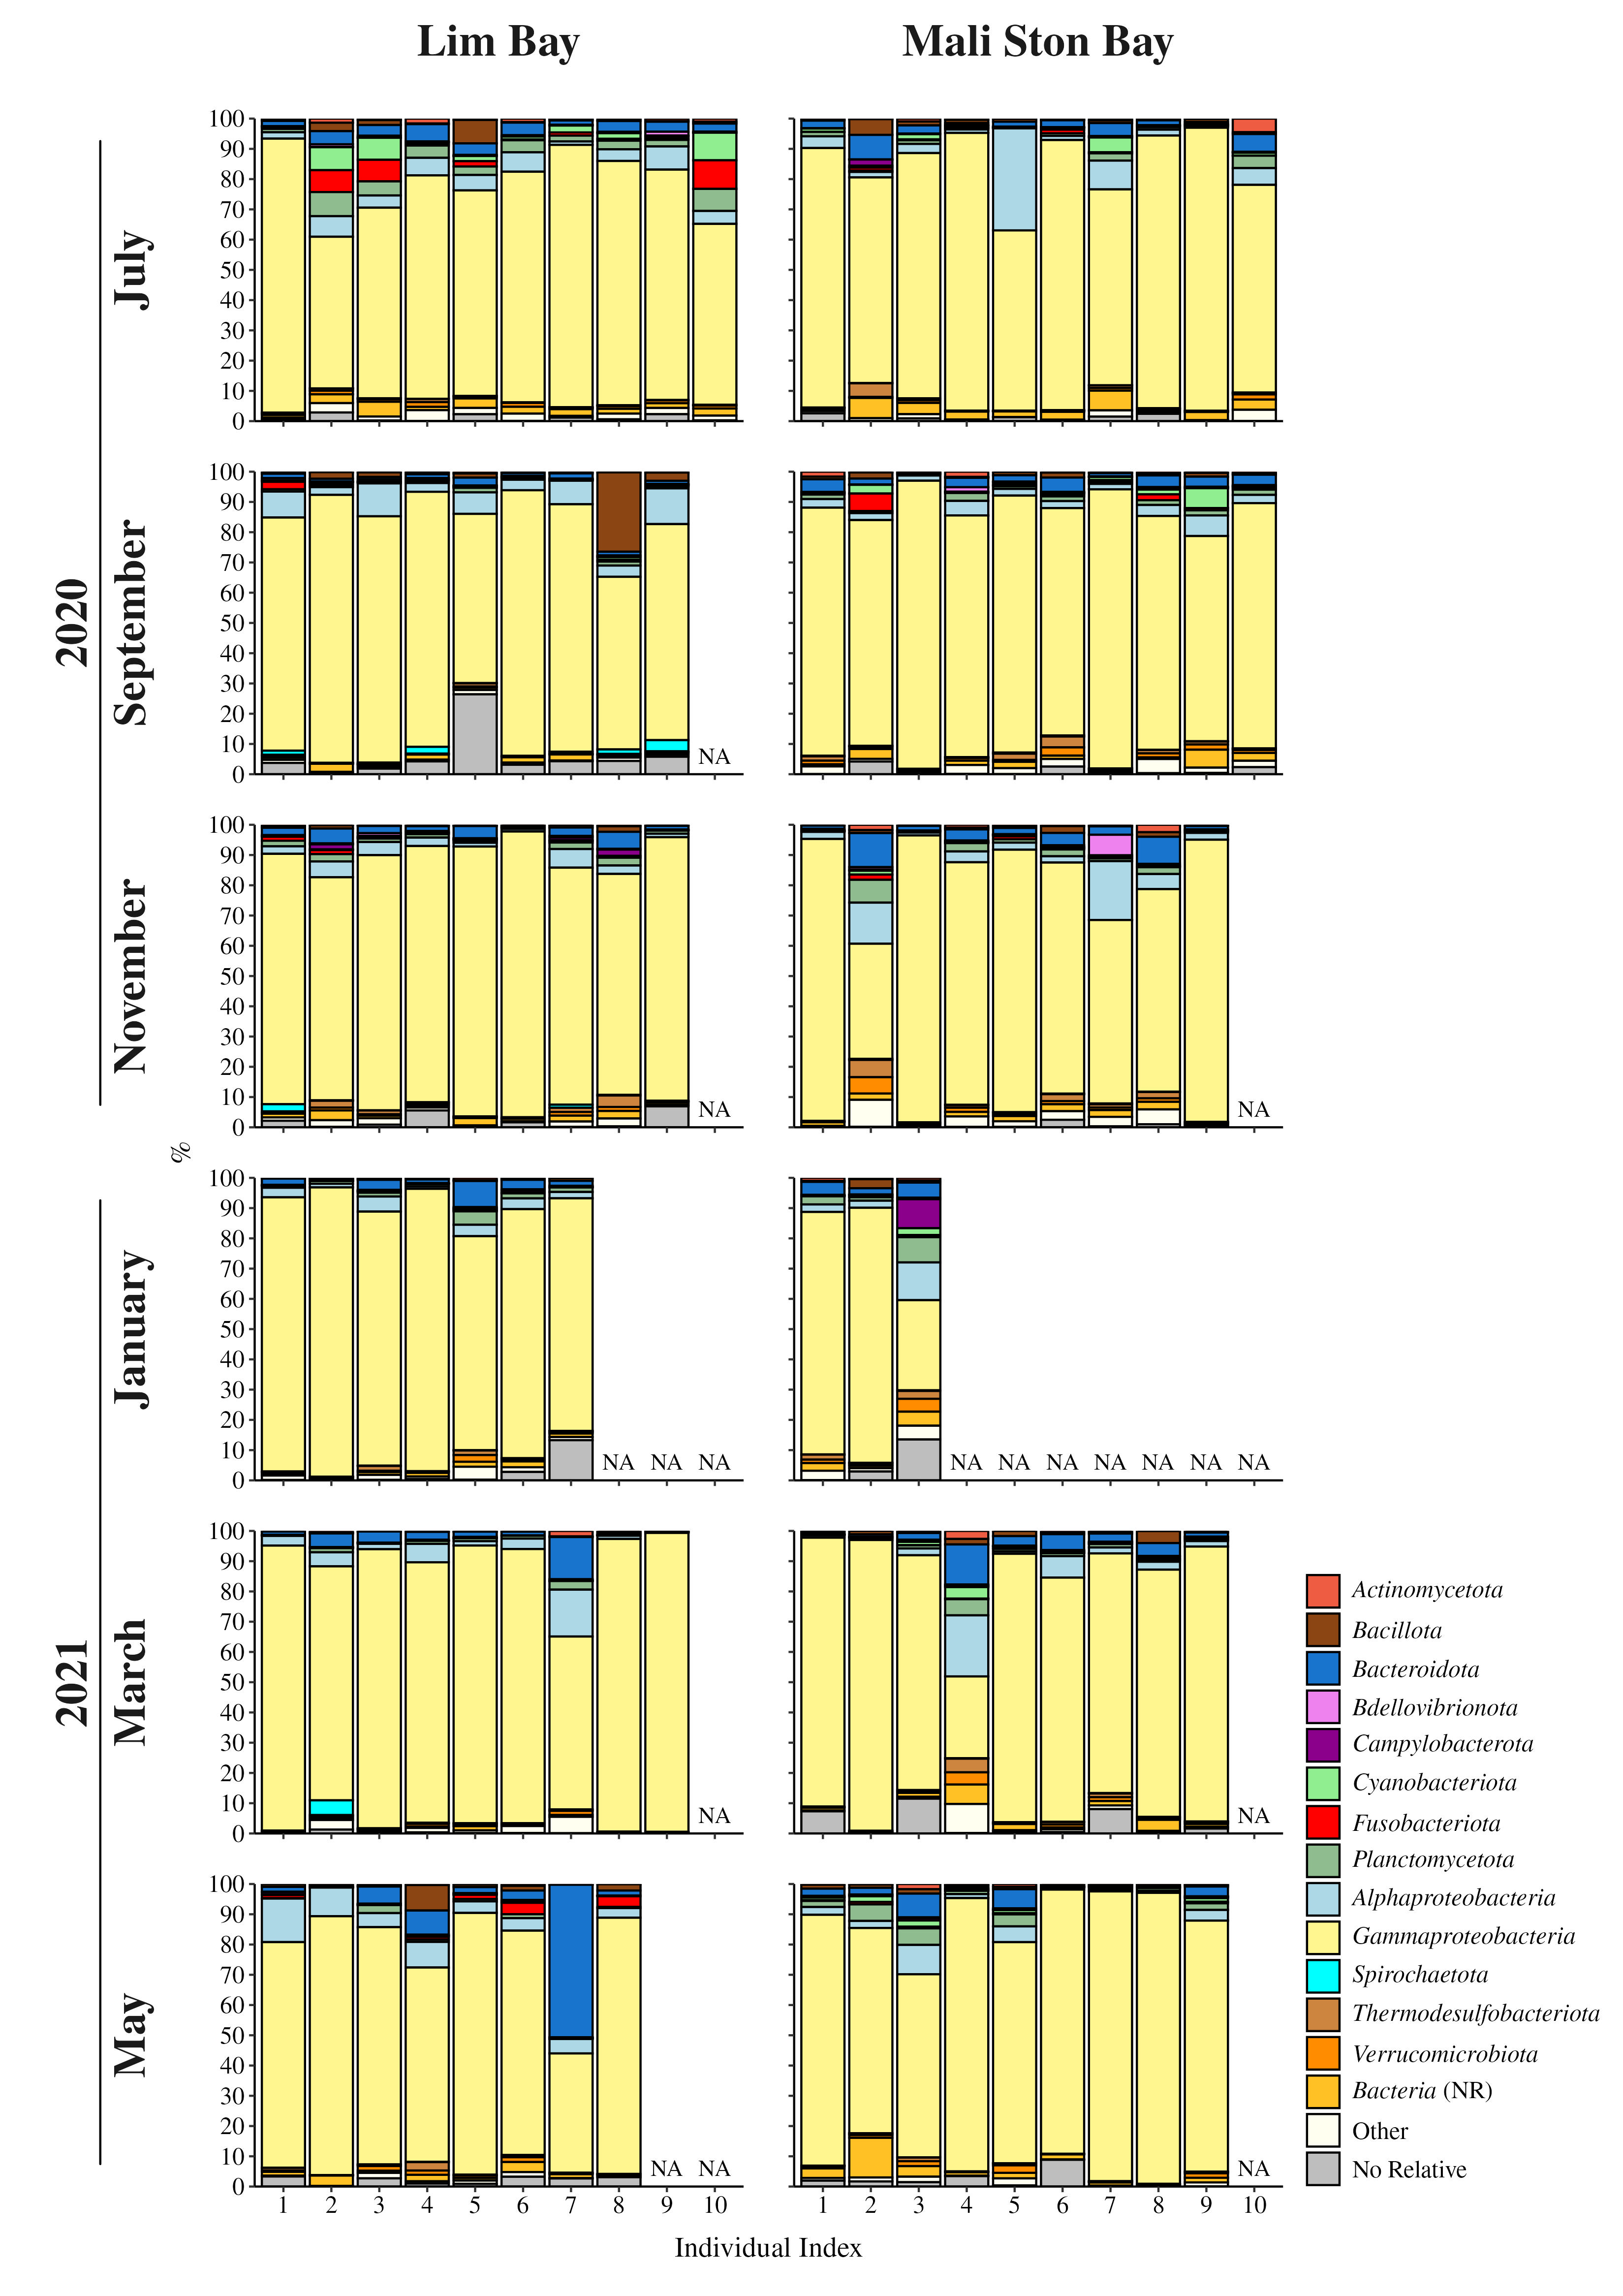
\includegraphics[width=0.8\linewidth]{../results/figures/taxonomy_gills_phylum} 

}

\caption{Taxonomic classification and relative contribution of the most abundant (\qty{>=3}{\percent}) bacterial and archaeal sequences from the gills of the mussel \emph{M. galloprovincialis} (gill microbiome). From July 2020 to May 2021, 10 mussels were collected per sampling month in Lim Bay and Mali Ston Bay. Each bar (individual index) represents an individual mussel. ``No Relative'' indicates sequences that could not be classified into any taxon, while ``NR'' (No Relative) next to the name of a taxonomic group refers to sequences that could not be assigned to any known taxon within that group. ``NA'' (Not Available) indicates samples that were not successfully analysed}\label{fig:taxonomy-gills-phylum}
\end{figure}



\subsection{Supplementary tables}\label{supplementary-tables}

% Begin the singlespace environment so that
% rows in the longtable are single spaced
\begin{singlespace}



\begingroup\fontsize{10}{12}\selectfont

\begin{longtable}[t]{ccccc>{\centering\arraybackslash}m{\textwidth / 11}>{\centering\arraybackslash}m{\textwidth / 11}}
\caption{\label{tab:nseq-notus-seawater-sediment}Sample ID, sampling date, location, and site, and the no. of sequences and OTUs for each sample from the seawater and sediment environment. The no. of sequences and OTUs was calculated after excluding sequences without known relatives, as well as eukaryotic, mitochondrial, and chloroplast sequences}\\
\toprule
\textbf{Sample ID} & \textbf{Environment} & \textbf{Date} & \textbf{Location} & \textbf{Site} & \textbf{No. of Sequences} & \textbf{No. of OTUs}\\
\midrule
\endfirsthead
\caption[]{\label{tab:nseq-notus-seawater-sediment}Sample ID, sampling date, location, and site, and the no. of sequences and OTUs for each sample from the seawater and sediment environment. The no. of sequences and OTUs was calculated after excluding sequences without known relatives, as well as eukaryotic, mitochondrial, and chloroplast sequences \textit{(continued)}}\\
\toprule
\textbf{Sample ID} & \textbf{Environment} & \textbf{Date} & \textbf{Location} & \textbf{Site} & \textbf{No. of Sequences} & \textbf{No. of OTUs}\\
\midrule
\endhead

\endfoot
\bottomrule
\endlastfoot
1 &  &  &  & Aquaculture & 3,037 & 390\\
\nopagebreak
2 & \multirow{-2}{*}{\centering\arraybackslash Seawater} & \multirow{-2}{*}{\centering\arraybackslash 10 July 2020} & \multirow{-2}{*}{\centering\arraybackslash Lim Bay} & Control & 3,193 & 408\\
\cmidrule{1-7}\pagebreak[0]
3 &  &  &  & Aquaculture & 7,309 & 389\\
\nopagebreak
4 & \multirow{-2}{*}{\centering\arraybackslash Seawater} & \multirow{-2}{*}{\centering\arraybackslash 7 July 2020} & \multirow{-2}{*}{\centering\arraybackslash Mali Ston Bay} & Control & 8,444 & 485\\
\cmidrule{1-7}\pagebreak[0]
5 &  &  &  & Aquaculture & 3,289 & 478\\
\nopagebreak
6 & \multirow{-2}{*}{\centering\arraybackslash Seawater} & \multirow{-2}{*}{\centering\arraybackslash 19 September 2020} & \multirow{-2}{*}{\centering\arraybackslash Lim Bay} & Control & 3,225 & 530\\
\cmidrule{1-7}\pagebreak[0]
7 &  &  &  & Aquaculture & 3,136 & 405\\
\nopagebreak
8 & \multirow{-2}{*}{\centering\arraybackslash Seawater} & \multirow{-2}{*}{\centering\arraybackslash 15 September 2020} & \multirow{-2}{*}{\centering\arraybackslash Mali Ston Bay} & Control & 3,212 & 438\\
\cmidrule{1-7}\pagebreak[0]
9 &  &  &  & Aquaculture & 2,376 & 449\\
\nopagebreak
10 & \multirow{-2}{*}{\centering\arraybackslash Seawater} & \multirow{-2}{*}{\centering\arraybackslash 14 November 2020} & \multirow{-2}{*}{\centering\arraybackslash Lim Bay} & Control & 2,959 & 480\\
\cmidrule{1-7}\pagebreak[0]
11 &  &  &  & Aquaculture & 2,931 & 459\\
\nopagebreak
12 & \multirow{-2}{*}{\centering\arraybackslash Seawater} & \multirow{-2}{*}{\centering\arraybackslash 10 November 2020} & \multirow{-2}{*}{\centering\arraybackslash Mali Ston Bay} & Control & 2,534 & 494\\
\cmidrule{1-7}\pagebreak[0]
13 &  &  &  & Aquaculture & 5,017 & 498\\
\nopagebreak
14 & \multirow{-2}{*}{\centering\arraybackslash Seawater} & \multirow{-2}{*}{\centering\arraybackslash 15 January 2021} & \multirow{-2}{*}{\centering\arraybackslash Lim Bay} & Control & 6,296 & 516\\
\cmidrule{1-7}\pagebreak[0]
15 &  &  &  & Aquaculture & 2,461 & 357\\
\nopagebreak
16 & \multirow{-2}{*}{\centering\arraybackslash Seawater} & \multirow{-2}{*}{\centering\arraybackslash 12 January 2021} & \multirow{-2}{*}{\centering\arraybackslash Mali Ston Bay} & Control & 2,772 & 413\\
\cmidrule{1-7}\pagebreak[0]
18 & Seawater & 18 March 2021 & Lim Bay & Control & 2,062 & 262\\
\cmidrule{1-7}\pagebreak[0]
19 &  &  &  & Aquaculture & 3,418 & 473\\
\nopagebreak
20 & \multirow{-2}{*}{\centering\arraybackslash Seawater} & \multirow{-2}{*}{\centering\arraybackslash 15 March 2021} & \multirow{-2}{*}{\centering\arraybackslash Mali Ston Bay} & Control & 2,952 & 518\\
\cmidrule{1-7}\pagebreak[0]
21 &  &  &  & Aquaculture & 5,169 & 281\\
\nopagebreak
22 & \multirow{-2}{*}{\centering\arraybackslash Seawater} & \multirow{-2}{*}{\centering\arraybackslash 7 May 2021} & \multirow{-2}{*}{\centering\arraybackslash Lim Bay} & Control & 4,186 & 293\\
\cmidrule{1-7}\pagebreak[0]
23 &  &  &  & Aquaculture & 5,188 & 550\\
\nopagebreak
24 & \multirow{-2}{*}{\centering\arraybackslash Seawater} & \multirow{-2}{*}{\centering\arraybackslash 3 May 2021} & \multirow{-2}{*}{\centering\arraybackslash Mali Ston Bay} & Control & 3,051 & 427\\
\cmidrule{1-7}\pagebreak[0]
25 &  &  &  & Aquaculture & 13,192 & 3,217\\
\nopagebreak
26 & \multirow{-2}{*}{\centering\arraybackslash Sediment} & \multirow{-2}{*}{\centering\arraybackslash 10 July 2020} & \multirow{-2}{*}{\centering\arraybackslash Lim Bay} & Control & 14,292 & 4,027\\
\cmidrule{1-7}\pagebreak[0]
27 &  &  &  & Aquaculture & 13,548 & 4,239\\
\nopagebreak
28 & \multirow{-2}{*}{\centering\arraybackslash Sediment} & \multirow{-2}{*}{\centering\arraybackslash 7 July 2020} & \multirow{-2}{*}{\centering\arraybackslash Mali Ston Bay} & Control & 7,194 & 2,722\\
\cmidrule{1-7}\pagebreak[0]
29 &  &  &  & Aquaculture & 19,217 & 4,006\\
\nopagebreak
30 & \multirow{-2}{*}{\centering\arraybackslash Sediment} & \multirow{-2}{*}{\centering\arraybackslash 19 September 2020} & \multirow{-2}{*}{\centering\arraybackslash Lim Bay} & Control & 20,879 & 4,444\\
\cmidrule{1-7}\pagebreak[0]
31 &  &  &  & Aquaculture & 30,251 & 3,708\\
\nopagebreak
32 & \multirow{-2}{*}{\centering\arraybackslash Sediment} & \multirow{-2}{*}{\centering\arraybackslash 15 September 2020} & \multirow{-2}{*}{\centering\arraybackslash Mali Ston Bay} & Control & 5,005 & 2,393\\
\cmidrule{1-7}\pagebreak[0]
33 &  &  &  & Aquaculture & 17,740 & 4,457\\
\nopagebreak
34 & \multirow{-2}{*}{\centering\arraybackslash Sediment} & \multirow{-2}{*}{\centering\arraybackslash 14 November 2020} & \multirow{-2}{*}{\centering\arraybackslash Lim Bay} & Control & 13,887 & 4,090\\
\cmidrule{1-7}\pagebreak[0]
35 &  &  &  & Aquaculture & 12,051 & 3,775\\
\nopagebreak
36 & \multirow{-2}{*}{\centering\arraybackslash Sediment} & \multirow{-2}{*}{\centering\arraybackslash 10 November 2020} & \multirow{-2}{*}{\centering\arraybackslash Mali Ston Bay} & Control & 6,888 & 3,047\\
\cmidrule{1-7}\pagebreak[0]
37 &  &  &  & Aquaculture & 17,320 & 4,387\\
\nopagebreak
38 & \multirow{-2}{*}{\centering\arraybackslash Sediment} & \multirow{-2}{*}{\centering\arraybackslash 15 January 2021} & \multirow{-2}{*}{\centering\arraybackslash Lim Bay} & Control & 10,657 & 3,699\\
\cmidrule{1-7}\pagebreak[0]
39 &  &  &  & Aquaculture & 21,574 & 4,439\\
\nopagebreak
40 & \multirow{-2}{*}{\centering\arraybackslash Sediment} & \multirow{-2}{*}{\centering\arraybackslash 12 January 2021} & \multirow{-2}{*}{\centering\arraybackslash Mali Ston Bay} & Control & 26,060 & 4,352\\
\cmidrule{1-7}\pagebreak[0]
41 &  &  &  & Aquaculture & 9,264 & 3,359\\
\nopagebreak
42 & \multirow{-2}{*}{\centering\arraybackslash Sediment} & \multirow{-2}{*}{\centering\arraybackslash 18 March 2021} & \multirow{-2}{*}{\centering\arraybackslash Lim Bay} & Control & 9,305 & 3,367\\
\cmidrule{1-7}\pagebreak[0]
43 &  &  &  & Aquaculture & 23,890 & 4,603\\
\nopagebreak
44 & \multirow{-2}{*}{\centering\arraybackslash Sediment} & \multirow{-2}{*}{\centering\arraybackslash 15 March 2021} & \multirow{-2}{*}{\centering\arraybackslash Mali Ston Bay} & Control & 8,902 & 3,358\\
\cmidrule{1-7}\pagebreak[0]
45 &  &  &  & Aquaculture & 12,116 & 4,046\\
\nopagebreak
46 & \multirow{-2}{*}{\centering\arraybackslash Sediment} & \multirow{-2}{*}{\centering\arraybackslash 7 May 2021} & \multirow{-2}{*}{\centering\arraybackslash Lim Bay} & Control & 13,380 & 4,295\\
\cmidrule{1-7}\pagebreak[0]
47 &  &  &  & Aquaculture & 12,924 & 3,595\\
\nopagebreak
48 & \multirow{-2}{*}{\centering\arraybackslash Sediment} & \multirow{-2}{*}{\centering\arraybackslash 3 May 2021} & \multirow{-2}{*}{\centering\arraybackslash Mali Ston Bay} & Control & 10,778 & 3,808\\*
\end{longtable}
\endgroup{}
\newpage



\begingroup\fontsize{10}{12}\selectfont

\begin{longtable}[t]{ccc>{\centering\arraybackslash}m{\textwidth / 11}>{\centering\arraybackslash}m{\textwidth / 11}>{\centering\arraybackslash}m{\textwidth / 11}>{\centering\arraybackslash}m{\textwidth / 11}}
\caption{\label{tab:nseq-notus-gills}Sample ID, sampling date and location, each individual ID and index, and the no. of sequences and OTUs for each gill sample of the mussel \emph{M. galloprovincialis} (gill microbiome). The no. of sequences and OTUs was calculated after excluding sequences without known relatives, as well as eukaryotic, mitochondrial, and chloroplast sequences}\\
\toprule
\textbf{Sample ID} & \textbf{Date} & \textbf{Location} & \textbf{Individual ID} & \textbf{Individual Index} & \textbf{No. of Sequences} & \textbf{No. of OTUs}\\
\midrule
\endfirsthead
\caption[]{\label{tab:nseq-notus-gills}Sample ID, sampling date and location, each individual ID and index, and the no. of sequences and OTUs for each gill sample of the mussel \emph{M. galloprovincialis} (gill microbiome). The no. of sequences and OTUs was calculated after excluding sequences without known relatives, as well as eukaryotic, mitochondrial, and chloroplast sequences \textit{(continued)}}\\
\toprule
\textbf{Sample ID} & \textbf{Date} & \textbf{Location} & \textbf{Individual ID} & \textbf{Individual Index} & \textbf{No. of Sequences} & \textbf{No. of OTUs}\\
\midrule
\endhead

\endfoot
\bottomrule
\endlastfoot
49 &  &  & 1 & 1 & 15,853 & 548\\
\nopagebreak
50 &  &  & 2 & 2 & 13,847 & 1,064\\
\nopagebreak
51 &  &  & 3 & 3 & 12,266 & 505\\
\nopagebreak
52 &  &  & 4 & 4 & 13,872 & 1,304\\
\nopagebreak
53 &  &  & 5 & 5 & 16,808 & 837\\
\nopagebreak
54 &  &  & 11 & 6 & 16,120 & 1,139\\
\nopagebreak
55 &  &  & 7 & 7 & 18,523 & 523\\
\nopagebreak
56 &  &  & 8 & 8 & 19,428 & 1,038\\
\nopagebreak
57 &  &  & 9 & 9 & 12,622 & 884\\
\nopagebreak
58 & \multirow{-10}{*}{\centering\arraybackslash 10 July 2020} & \multirow{-10}{*}{\centering\arraybackslash Lim Bay} & 10 & 10 & 14,824 & 1,022\\
\cmidrule{1-7}\pagebreak[0]
59 &  &  & 1 & 1 & 14,800 & 673\\
\nopagebreak
60 &  &  & 2 & 2 & 13,186 & 485\\
\nopagebreak
61 &  &  & 3 & 3 & 15,035 & 731\\
\nopagebreak
62 &  &  & 4 & 4 & 14,465 & 320\\
\nopagebreak
63 &  &  & 5 & 5 & 12,768 & 191\\
\nopagebreak
64 &  &  & 6 & 6 & 15,414 & 425\\
\nopagebreak
65 &  &  & 7 & 7 & 12,619 & 734\\
\nopagebreak
66 &  &  & 8 & 8 & 14,380 & 457\\
\nopagebreak
67 &  &  & 9 & 9 & 14,044 & 262\\
\nopagebreak
68 & \multirow{-10}{*}{\centering\arraybackslash 7 July 2020} & \multirow{-10}{*}{\centering\arraybackslash Mali Ston Bay} & 10 & 10 & 14,292 & 1,229\\
\cmidrule{1-7}\pagebreak[0]
69 &  &  & 1 & 1 & 14,607 & 559\\
\nopagebreak
71 &  &  & 3 & 2 & 12,319 & 272\\
\nopagebreak
72 &  &  & 4 & 3 & 11,897 & 324\\
\nopagebreak
73 &  &  & 5 & 4 & 11,957 & 431\\
\nopagebreak
74 &  &  & 6 & 5 & 8,633 & 647\\
\nopagebreak
75 &  &  & 7 & 6 & 10,208 & 443\\
\nopagebreak
76 &  &  & 8 & 7 & 60,611 & 601\\
\nopagebreak
77 &  &  & 9 & 8 & 14,719 & 603\\
\nopagebreak
78 & \multirow{-9}{*}{\centering\arraybackslash 19 September 2020} & \multirow{-9}{*}{\centering\arraybackslash Lim Bay} & 10 & 9 & 12,249 & 434\\
\cmidrule{1-7}\pagebreak[0]
79 &  &  & 1 & 1 & 15,175 & 866\\
\nopagebreak
80 &  &  & 2 & 2 & 14,029 & 525\\
\nopagebreak
81 &  &  & 3 & 3 & 14,641 & 299\\
\nopagebreak
82 &  &  & 4 & 4 & 13,308 & 858\\
\nopagebreak
83 &  &  & 5 & 5 & 15,088 & 617\\
\nopagebreak
84 &  &  & 6 & 6 & 16,943 & 1,076\\
\nopagebreak
85 &  &  & 7 & 7 & 17,061 & 491\\
\nopagebreak
86 &  &  & 8 & 8 & 17,856 & 888\\
\nopagebreak
87 &  &  & 9 & 9 & 14,753 & 794\\
\nopagebreak
88 & \multirow{-10}{*}{\centering\arraybackslash 15 September 2020} & \multirow{-10}{*}{\centering\arraybackslash Mali Ston Bay} & 10 & 10 & 15,466 & 927\\
\cmidrule{1-7}\pagebreak[0]
89 &  &  & 1 & 1 & 13,090 & 600\\
\nopagebreak
90 &  &  & 2 & 2 & 14,861 & 814\\
\nopagebreak
91 &  &  & 3 & 3 & 16,309 & 508\\
\nopagebreak
92 &  &  & 4 & 4 & 12,120 & 463\\
\nopagebreak
93 &  &  & 5 & 5 & 18,244 & 404\\
\nopagebreak
95 &  &  & 7 & 6 & 14,538 & 204\\
\nopagebreak
96 &  &  & 8 & 7 & 14,815 & 865\\
\nopagebreak
97 &  &  & 9 & 8 & 15,054 & 1,030\\
\nopagebreak
98 & \multirow{-9}{*}{\centering\arraybackslash 14 November 2020} & \multirow{-9}{*}{\centering\arraybackslash Lim Bay} & 10 & 9 & 11,746 & 300\\
\cmidrule{1-7}\pagebreak[0]
99 &  &  & 1 & 1 & 12,990 & 321\\
\nopagebreak
100 &  &  & 2 & 2 & 15,906 & 2,488\\
\nopagebreak
101 &  &  & 3 & 3 & 17,187 & 363\\
\nopagebreak
103 &  &  & 5 & 4 & 14,867 & 1,157\\
\nopagebreak
104 &  &  & 11 & 5 & 15,278 & 760\\
\nopagebreak
105 &  &  & 7 & 6 & 15,171 & 1,058\\
\nopagebreak
106 &  &  & 8 & 7 & 12,428 & 697\\
\nopagebreak
107 &  &  & 9 & 8 & 16,821 & 1,309\\
\nopagebreak
108 & \multirow{-9}{*}{\centering\arraybackslash 10 November 2020} & \multirow{-9}{*}{\centering\arraybackslash Mali Ston Bay} & 10 & 9 & 14,874 & 349\\
\cmidrule{1-7}\pagebreak[0]
109 &  &  & 1 & 1 & 39,148 & 857\\
\nopagebreak
111 &  &  & 3 & 2 & 35,902 & 696\\
\nopagebreak
112 &  &  & 4 & 3 & 33,282 & 1,241\\
\nopagebreak
113 &  &  & 5 & 4 & 28,265 & 707\\
\nopagebreak
114 &  &  & 6 & 5 & 32,692 & 2,248\\
\nopagebreak
115 &  &  & 7 & 6 & 32,932 & 1,284\\
\nopagebreak
116 & \multirow{-7}{*}{\centering\arraybackslash 15 January 2021} & \multirow{-7}{*}{\centering\arraybackslash Lim Bay} & 8 & 7 & 32,762 & 1,099\\
\cmidrule{1-7}\pagebreak[0]
125 &  &  & 7 & 1 & 17,689 & 1,131\\
\nopagebreak
127 &  &  & 9 & 2 & 17,488 & 685\\
\nopagebreak
128 & \multirow{-3}{*}{\centering\arraybackslash 12 January 2021} & \multirow{-3}{*}{\centering\arraybackslash Mali Ston Bay} & 10 & 3 & 17,378 & 2,025\\
\cmidrule{1-7}\pagebreak[0]
129 &  &  & 11 & 1 & 12,564 & 225\\
\nopagebreak
130 &  &  & 12 & 2 & 8,908 & 628\\
\nopagebreak
131 &  &  & 3 & 3 & 11,939 & 282\\
\nopagebreak
132 &  &  & 4 & 4 & 16,016 & 592\\
\nopagebreak
133 &  &  & 5 & 5 & 8,540 & 374\\
\nopagebreak
135 &  &  & 7 & 6 & 9,198 & 351\\
\nopagebreak
136 &  &  & 8 & 7 & 11,089 & 1,197\\
\nopagebreak
137 &  &  & 9 & 8 & 10,472 & 160\\
\nopagebreak
138 & \multirow{-9}{*}{\centering\arraybackslash 18 March 2021} & \multirow{-9}{*}{\centering\arraybackslash Lim Bay} & 10 & 9 & 10,986 & 93\\
\cmidrule{1-7}\pagebreak[0]
139 &  &  & 1 & 1 & 13,123 & 287\\
\nopagebreak
140 &  &  & 2 & 2 & 16,109 & 210\\
\nopagebreak
141 &  &  & 3 & 3 & 15,072 & 490\\
\nopagebreak
143 &  &  & 5 & 4 & 9,533 & 1,561\\
\nopagebreak
144 &  &  & 6 & 5 & 11,426 & 356\\
\nopagebreak
145 &  &  & 7 & 6 & 15,174 & 702\\
\nopagebreak
146 &  &  & 8 & 7 & 16,144 & 882\\
\nopagebreak
147 &  &  & 9 & 8 & 15,148 & 506\\
\nopagebreak
148 & \multirow{-9}{*}{\centering\arraybackslash 15 March 2021} & \multirow{-9}{*}{\centering\arraybackslash Mali Ston Bay} & 10 & 9 & 9,495 & 350\\
\cmidrule{1-7}\pagebreak[0]
149 &  &  & 1 & 1 & 14,563 & 293\\
\nopagebreak
151 &  &  & 3 & 2 & 17,581 & 185\\
\nopagebreak
152 &  &  & 4 & 3 & 16,798 & 1,069\\
\nopagebreak
153 &  &  & 5 & 4 & 15,356 & 488\\
\nopagebreak
154 &  &  & 6 & 5 & 18,075 & 625\\
\nopagebreak
155 &  &  & 7 & 6 & 26,405 & 926\\
\nopagebreak
156 &  &  & 8 & 7 & 24,010 & 265\\
\nopagebreak
157 & \multirow{-8}{*}{\centering\arraybackslash 7 May 2021} & \multirow{-8}{*}{\centering\arraybackslash Lim Bay} & 9 & 8 & 29,240 & 327\\
\cmidrule{1-7}\pagebreak[0]
159 &  &  & 1 & 1 & 18,499 & 547\\
\nopagebreak
160 &  &  & 2 & 2 & 22,381 & 848\\
\nopagebreak
161 &  &  & 3 & 3 & 12,097 & 782\\
\nopagebreak
162 &  &  & 4 & 4 & 13,295 & 219\\
\nopagebreak
163 &  &  & 5 & 5 & 13,295 & 1,056\\
\nopagebreak
164 &  &  & 6 & 6 & 15,082 & 193\\
\nopagebreak
165 &  &  & 7 & 7 & 16,106 & 277\\
\nopagebreak
167 &  &  & 9 & 8 & 19,715 & 320\\
\nopagebreak
168 & \multirow{-9}{*}{\centering\arraybackslash 3 May 2021} & \multirow{-9}{*}{\centering\arraybackslash Mali Ston Bay} & 10 & 9 & 14,766 & 802\\*
\end{longtable}
\endgroup{}
\newpage



\begingroup\fontsize{10}{12}\selectfont

\begin{longtable}[t]{>{\centering\arraybackslash}m{\textwidth / 8}>{\centering\arraybackslash}m{\textwidth / 16}>{\centering\arraybackslash}m{\textwidth / 16}>{\centering\arraybackslash}m{\textwidth / 16}>{\centering\arraybackslash}m{\textwidth / \real{2.3}}>{\centering\arraybackslash}m{\textwidth / 16}}
\caption{\label{tab:kruskal-wallis}The statistics of richness estimator and diversity index parameters of microbial communities from different environments and sites. Parameters were tested with the Kruskal-Wallis \emph{H} test followed by pairwise comparisons using the Mann-Whitney \emph{U} test. Bonferroni correction was applied to address the problem of multiple comparisons}\\
\toprule
\multicolumn{1}{c}{\textbf{}} & \multicolumn{3}{c}{\textbf{Kruskal-Wallis \textit{H} test}} & \multicolumn{2}{c}{\textbf{Mann-Whitney \textit{U} test}} \\
\cmidrule(l{3pt}r{3pt}){2-4} \cmidrule(l{3pt}r{3pt}){5-6}
\textbf{Parameter} & \textbf{\textit{H}} & \textbf{\textit{df}} & \textbf{\textit{p}} & \textbf{Comparisons Between Environments and Sites} & \textbf{\textit{p}}\\
\midrule
\endfirsthead
\caption[]{\label{tab:kruskal-wallis}The statistics of richness estimator and diversity index parameters of microbial communities from different environments and sites. Parameters were tested with the Kruskal-Wallis \emph{H} test followed by pairwise comparisons using the Mann-Whitney \emph{U} test. Bonferroni correction was applied to address the problem of multiple comparisons \textit{(continued)}}\\
\toprule
\multicolumn{1}{c}{\textbf{}} & \multicolumn{3}{c}{\textbf{Kruskal-Wallis \textit{H} test}} & \multicolumn{2}{c}{\textbf{Mann-Whitney \textit{U} test}} \\
\cmidrule(l{3pt}r{3pt}){2-4} \cmidrule(l{3pt}r{3pt}){5-6}
\textbf{Parameter} & \textbf{\textit{H}} & \textbf{\textit{df}} & \textbf{\textit{p}} & \textbf{Comparisons Between Environments and Sites} & \textbf{\textit{p}}\\
\midrule
\endhead

\endfoot
\bottomrule
\endlastfoot
 &  &  &  & Seawater (Aquaculture)–Sediment (Aquaculture) & <0.0001\\
\nopagebreak
 &  &  &  & Seawater (Aquaculture)–Gills (Aquaculture) & <0.01\\
\nopagebreak
 &  &  &  & Seawater (Aquaculture)–Seawater (Control) & 1.00\\
\nopagebreak
 &  &  &  & Seawater (Aquaculture)–Sediment (Control) & <0.0001\\
\nopagebreak
 &  &  &  & Sediment (Aquaculture)–Gills (Aquaculture) & <0.0001\\
\nopagebreak
 &  &  &  & Sediment (Aquaculture)–Seawater (Control) & <0.0001\\
\nopagebreak
 &  &  &  & Sediment (Aquaculture)–Sediment (Control) & 0.60\\
\nopagebreak
 &  &  &  & Gills (Aquaculture)–Seawater (Control) & <0.001\\
\nopagebreak
 &  &  &  & Gills (Aquaculture)–Sediment (Control) & <0.0001\\
\nopagebreak
\multirow{-10}{\textwidth / 8}{\centering\arraybackslash Observed No. of OTUs} & \multirow{-10}{\textwidth / 16}{\centering\arraybackslash 79.1} & \multirow{-10}{\textwidth / 16}{\centering\arraybackslash 4} & \multirow{-10}{\textwidth / 16}{\centering\arraybackslash <0.0001} & Seawater (Control)–Sediment (Control) & <0.0001\\
\cmidrule{1-6}\pagebreak[0]
 &  &  &  & Seawater (Aquaculture)–Sediment (Aquaculture) & <0.0001\\
\nopagebreak
 &  &  &  & Seawater (Aquaculture)–Gills (Aquaculture) & 1.00\\
\nopagebreak
 &  &  &  & Seawater (Aquaculture)–Seawater (Control) & 1.00\\
\nopagebreak
 &  &  &  & Seawater (Aquaculture)–Sediment (Control) & <0.0001\\
\nopagebreak
 &  &  &  & Sediment (Aquaculture)–Gills (Aquaculture) & <0.0001\\
\nopagebreak
 &  &  &  & Sediment (Aquaculture)–Seawater (Control) & <0.0001\\
\nopagebreak
 &  &  &  & Sediment (Aquaculture)–Sediment (Control) & 1.00\\
\nopagebreak
 &  &  &  & Gills (Aquaculture)–Seawater (Control) & 1.00\\
\nopagebreak
 &  &  &  & Gills (Aquaculture)–Sediment (Control) & <0.0001\\
\nopagebreak
\multirow{-10}{\textwidth / 8}{\centering\arraybackslash Chao1} & \multirow{-10}{\textwidth / 16}{\centering\arraybackslash 60.3} & \multirow{-10}{\textwidth / 16}{\centering\arraybackslash 4} & \multirow{-10}{\textwidth / 16}{\centering\arraybackslash <0.0001} & Seawater (Control)–Sediment (Control) & <0.0001\\
\cmidrule{1-6}\pagebreak[0]
 &  &  &  & Seawater (Aquaculture)–Sediment (Aquaculture) & <0.0001\\
\nopagebreak
 &  &  &  & Seawater (Aquaculture)–Gills (Aquaculture) & 1.00\\
\nopagebreak
 &  &  &  & Seawater (Aquaculture)–Seawater (Control) & 1.00\\
\nopagebreak
 &  &  &  & Seawater (Aquaculture)–Sediment (Control) & <0.0001\\
\nopagebreak
 &  &  &  & Sediment (Aquaculture)–Gills (Aquaculture) & <0.0001\\
\nopagebreak
 &  &  &  & Sediment (Aquaculture)–Seawater (Control) & <0.0001\\
\nopagebreak
 &  &  &  & Sediment (Aquaculture)–Sediment (Control) & 1.00\\
\nopagebreak
 &  &  &  & Gills (Aquaculture)–Seawater (Control) & 1.00\\
\nopagebreak
 &  &  &  & Gills (Aquaculture)–Sediment (Control) & <0.0001\\
\nopagebreak
\multirow{-10}{\textwidth / 8}{\centering\arraybackslash ACE} & \multirow{-10}{\textwidth / 16}{\centering\arraybackslash 60.0} & \multirow{-10}{\textwidth / 16}{\centering\arraybackslash 4} & \multirow{-10}{\textwidth / 16}{\centering\arraybackslash <0.0001} & Seawater (Control)–Sediment (Control) & <0.0001\\
\cmidrule{1-6}\pagebreak[0]
 &  &  &  & Seawater (Aquaculture)–Sediment (Aquaculture) & <0.0001\\
\nopagebreak
 &  &  &  & Seawater (Aquaculture)–Gills (Aquaculture) & <0.0001\\
\nopagebreak
 &  &  &  & Seawater (Aquaculture)–Seawater (Control) & 1.00\\
\nopagebreak
 &  &  &  & Seawater (Aquaculture)–Sediment (Control) & <0.0001\\
\nopagebreak
 &  &  &  & Sediment (Aquaculture)–Gills (Aquaculture) & <0.0001\\
\nopagebreak
 &  &  &  & Sediment (Aquaculture)–Seawater (Control) & <0.0001\\
\nopagebreak
 &  &  &  & Sediment (Aquaculture)–Sediment (Control) & 0.68\\
\nopagebreak
 &  &  &  & Gills (Aquaculture)–Seawater (Control) & <0.0001\\
\nopagebreak
 &  &  &  & Gills (Aquaculture)–Sediment (Control) & <0.0001\\
\nopagebreak
\multirow{-10}{\textwidth / 8}{\centering\arraybackslash Exponential Shannon} & \multirow{-10}{\textwidth / 16}{\centering\arraybackslash 93.8} & \multirow{-10}{\textwidth / 16}{\centering\arraybackslash 4} & \multirow{-10}{\textwidth / 16}{\centering\arraybackslash <0.0001} & Seawater (Control)–Sediment (Control) & <0.0001\\
\cmidrule{1-6}\pagebreak[0]
 &  &  &  & Seawater (Aquaculture)–Sediment (Aquaculture) & <0.0001\\
\nopagebreak
 &  &  &  & Seawater (Aquaculture)–Gills (Aquaculture) & <0.0001\\
\nopagebreak
 &  &  &  & Seawater (Aquaculture)–Seawater (Control) & 1.00\\
\nopagebreak
 &  &  &  & Seawater (Aquaculture)–Sediment (Control) & <0.0001\\
\nopagebreak
 &  &  &  & Sediment (Aquaculture)–Gills (Aquaculture) & <0.0001\\
\nopagebreak
 &  &  &  & Sediment (Aquaculture)–Seawater (Control) & <0.0001\\
\nopagebreak
 &  &  &  & Sediment (Aquaculture)–Sediment (Control) & 1.00\\
\nopagebreak
 &  &  &  & Gills (Aquaculture)–Seawater (Control) & <0.0001\\
\nopagebreak
 &  &  &  & Gills (Aquaculture)–Sediment (Control) & <0.0001\\
\nopagebreak
\multirow{-10}{\textwidth / 8}{\centering\arraybackslash Inverse Simpson} & \multirow{-10}{\textwidth / 16}{\centering\arraybackslash 95.5} & \multirow{-10}{\textwidth / 16}{\centering\arraybackslash 4} & \multirow{-10}{\textwidth / 16}{\centering\arraybackslash <0.0001} & Seawater (Control)–Sediment (Control) & <0.0001\\*
\end{longtable}
\endgroup{}

% End the singlespace environment
\end{singlespace}

\end{document}
